\documentclass{article}
\usepackage[utf8]{inputenc}

\title{Interacting Particle System Thesis}
\author{Stefan Eng}
\date{2019/2020}

\usepackage{amsthm}
\usepackage{amssymb}
\usepackage{amsmath}
\usepackage{hyperref}
\usepackage{caption}
\usepackage{mathrsfs}
\usepackage{blkarray}

\usepackage{natbib}
\usepackage{graphicx}

\usepackage{tikz}
\usetikzlibrary{calc, automata, chains, arrows.meta}


\theoremstyle{plain}
\newtheorem{theorem}{Theorem}[section]
\newtheorem{example}{Example}[section]
\newtheorem{lemma}{Lemma}[section]
\newtheorem{prop}{Proposition}[section]

\theoremstyle{definition}
\newtheorem{defn}{Definition}[section]
\newtheorem{exercise}{Exercise}[section]

\theoremstyle{remark}
\newtheorem*{note}{Note}
\newtheorem*{remark}{Remark}

\newcommand{\R}{\mathbb{R}}
\newcommand{\Rs}{\mathcal{R}}
\newcommand{\Gs}{\mathcal{G}}
\newcommand{\Cs}{\mathcal{C}}
\newcommand{\Q}{\mathbb{Q}}
\newcommand{\A}{\mathcal{A}}
\newcommand{\F}{\mathcal{F}}
\newcommand{\E}{\mathcal{E}}
\newcommand{\M}{\mathcal{M}}
\newcommand{\N}{\mathcal{N}}
\newcommand{\Z}{\mathbb{Z}}
\newcommand{\Zs}{{\{0,1\}^\mathbb{Z}}}
\newcommand{\I}{\mathcal{I}}
\newcommand{\D}{\mathcal{D}}
\newcommand{\B}{{\mathcal{B}_{\mathbb{R}}}}
\newcommand{\BU}{{\mathcal{B}_{[0,1]}}}
\newcommand{\loc}{L_{\text{loc}}^1}
\newcommand{\powset}{\mathcal{P}}
\newcommand{\outm}{\mu^{*}}
\newcommand{\cdict}{\Rightarrow\!\Leftarrow}
\newcommand{\Var}{\operatorname {Var}}

% X_1, ..., X_n
\newcommand{\Xn}{\ensuremath{X_1,\ldots,X_n}}
\newcommand{\xn}{\ensuremath{x_1,\ldots,x_n}}

\begin{document}

\maketitle

\section{Introduction}

\section{Preliminaries}

\section{Stochastic Processes}

\section{Percolation}

\section{Interacting Particle Systems}

\subsection{Contact Process}

\subsection{Two node contact process}

Define a contact process on the finite graph with two nodes and one edge between them.

\begin{align}
    1 &\to 0 \text{ at rate } 1\\
    0 &\to 1 \text{ at rate } \begin{cases}
        \lambda & \text{ if neighbor is 1}\\
        0 & \text{ otherwise}
    \end{cases}
\end{align}

Start the process with both nodes at 1.
Clearly we will eventually reach $(0,0)$.
We can express the $Q$ matrix as

% Info on blockarray
% https://tex.stackexchange.com/a/59519/41827
$$
Q = \begin{blockarray}{ccccc}
    & (1,1) & (1,0) & (0,1) & (0,0)\\
    \begin{block}{c(cccc)}
        (1,1) & -2 & 1 & 1 & 0\\
        (1,0) & \lambda & - 1 - \lambda & 0 & 1\\
        (0,1) & \lambda & 0 & - 1 - \lambda & 1\\
        (0,0) & 0 & 0 & 0 & 0\\
    \end{block}
\end{blockarray}
$$
which is equivalent to combining the two nodes $(1,0)$ and $(0,1)$, which we will now call $(1,0)$.
This new node will have a rate of 2. TODO: Explain why?
$$
Q = \begin{blockarray}{cccc}
    & (1,1) & (0,1) & (0,0)\\
    \begin{block}{c(ccc)}
        (1,1) & -2 & 2 & 0\\
        (1,0) & \lambda & - 1 - \lambda & 1\\
        (0,0) & 0 & 0 & 0\\
    \end{block}
\end{blockarray}
$$


\begin{figure}
    \centering
   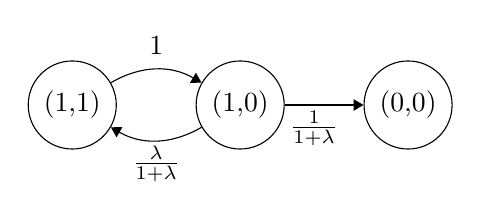
\begin{tikzpicture}[start chain = going right,
   -Triangle, every loop/.append style = {-Triangle}]
   \node[state, on chain]  (0) {(1,1)};
   \node[state, on chain]  (1) {(1,0)};
   \node[state, on chain]  (2) {(0,0)};
   
   % TODO: Need to add labels
   \draw (0) edge[bend left] node[yshift=3mm]{$1$} (1);
   \draw (1) edge[bend left] node[yshift=-3mm]{$\frac{\lambda}{1 + \lambda}$}(0);
   \draw (1) edge[left] node[xshift=3mm, yshift=-3mm]{$\frac{1}{1 + \lambda}$} (2);
   
   
   %\foreach \i in {0,...,2} 
%     \node[state, on chain]  (\i) {\i};
 %  \foreach \i in {0,...,} {
  %   \draw let \n1 = { int(\i+1) } in
   %    (\i)  edge[bend left] (\n1)
    %   (\n1) edge[bend left] (\i);
   %}
   %\foreach \i in {1,...,3}
    % \draw  (\i) edge[loop below] (\i);
   %draw    (0)  edge[loop left]   (0);
   %\draw    (4)  edge[loop right]  (4);
\end{tikzpicture}
    \caption{Embedded discrete Markov chain for two node contact process}
    \label{fig:discrete_mc_two_contact}
\end{figure}

Let $T_\lambda$ be the time in which we hit $(0,0)$.
The wait time while in node $(1,1)$ is exponentially distributed with parameter $- q_{(1,1)} = 2$ and similarly the wait time while in node $(1,0)$ or $(0,1)$ is exponentially distributed with parameter $- q_{(1,0)} = 1 + \lambda$.

Let $N$ be the number of times that the process wait at node $(1,0)$. Equivalently, it one more than the number of loops the discrete chain does from $(1,0) \to (1,1) \to (1,0)$. TODO: Need to modivate this better...
$$
P(N = n) = \left(\frac{\lambda}{1 + \lambda} \right)^{n - 1} \frac{1}{1 + \lambda} \quad n = 1,2,\ldots
$$
with
\begin{align*}
    E[N] &= 1 + \lambda\\
    \Var(N) &= \frac{\lambda/(1 + \lambda)}{1/(1 + \lambda)^2} = \lambda (1 + \lambda)
\end{align*}


Let $X_1, X_2, \ldots$ be iid random variables with $X_i \sim \exp(2) + \exp(1 + \lambda)$, which denotes the wait time for one loop. Since the wait times are independent, then 
$$
E[X_i] = \frac{1}{2} + \frac{1}{1 + \lambda} = \frac{3 + \lambda}{2(1 + \lambda)}
$$

Now we can express $T_\lambda$ as a random sum
$$
T_\lambda = \sum_{i = 1}^N X_i
$$

Using the theory of random sums \cite{Ross97}, we have that
$$
E[T_\lambda] = E\left[ \sum_{i = 1}^N X_i \right] = E[X_1] E[N] = \frac{3 + \lambda}{2(1 + \lambda)} \cdot (1 + \lambda)
$$

Also, the variance of a random sum is defined as
\begin{align*}
    \Var\left( \sum_{i = 1}^N X_i \right) &= E[N]\Var(X) + (E[X])^2 \Var(N)\\
    &= (1 + \lambda) \frac{(1 + \lambda)^2 + 4}{4(1 + \lambda)^2} + \frac{(3 + \lambda)^2}{4 (1 + \lambda)^2} \lambda (1 + \lambda)^2\\
    &= \frac{\lambda^3 + 8 \lambda^2 + 17 \lambda + 14}{4(1 + \lambda)}\\
    &= \frac{\lambda^2 + 7 \lambda + 10}{4} + \frac{1}{1 + \lambda}
\end{align*}

\subsubsection{Finite State Space}
Assume that the state space is finite, e.g. $X = \{ 0,1 \}^{\Z / n}$.
Each state $i$ is connected to its neighbor $i - 1 \mod n$ and $i + i \mod n$.

\subsubsection{Graphical Representation}

\subsection{Voter Model}

Questions/Exercises to answer from \cite{steif1991}.
\begin{enumerate}
    \item In 1 dimension from $\mu_\theta$,
    $$
    P(\eta_t(x) \not = \eta_t(x + 1)) \sim \frac{c}{\sqrt{t}}
    $$
    Does this imply
    $$
    P(\eta_t(x) = \eta_t(x + 1), \forall t \geq T) \quad T \to \infty
    $$
    \item Show that starting with $\mu_{1/2}$ ...  ??? Can't read the notes
    \item In 2-dim starting from $\mu_\theta$
        $$
    P(\eta_t(x) \not = \eta_t(x + 1)) \sim \frac{c}{\log{t}}
    $$
    (This uses highly non-trivial facts about random walks in 2-dimensions)
    \item In $d \geq 3$, what type of correlations does $\nu$ have?
    In other words, does
    $$
    E^{\nu_\theta}[\eta(x) \eta(y)] - E^{\nu_\theta}[\eta(x)] E^{\nu_\theta}[\eta(y)] \longrightarrow 0 \quad \text{as } |x - y| \to \infty
    $$
    If so, at what rate? Exponential? Power law? Take $\theta = 1/2$ for simplicity.
\end{enumerate}

\section{Statistical Mechanics}

\begin{defn}[Entropy]
    The entropy of a discrete random variable $X$ is given by
    $$
    H(X) = -E[\log(P(X))]
    $$
    where $P$ is the probability distribution function of $X$.
\end{defn}

\begin{theorem}
The entropy of a discrete random variable is maximized at the uniform distribution where the entropy is $\log |S|$
\end{theorem}

\begin{proof}
TODO: Jenson's inequality
\end{proof}

\bibliographystyle{plainnat}
\bibliography{references}
\end{document}
